\documentclass[english,10pt,twocolumn]{article}

\usepackage[T1]{fontenc}
\usepackage{times}
\usepackage{fullpage}
\usepackage{babel}
\usepackage{graphicx}
\usepackage{tikz}
\usepackage{pgfplots}
\usepackage{caption}


\begin{document}

\title{Keyvee: A Unikernel Key-Value Store}
\author{\
Nate Brennand\\nsb2142@colmbia.edu
\and
Gudbergur Erlendsson\\ge2187@columbia.edu
\and
Mishail Tupas\\mlt2156@columbia.edu}
\date{May 8, 2015}
\maketitle
\thispagestyle{empty}


\begin{abstract}
Traditional web infrastructures consist of a cluster of virtual machines running a full operating system like Linux or a BSD variant.
This provides a simple consistent platform for developers to write their applications against but running a full stack machine on top of hypervisors is understandable in an historical context but it is not neccesarily the most efficient.
One downside for example is extra overhead that we propose can be eliminated.
Key-value datastores are a common component of web infrastructure for various use cases, the most prominent one being Redis.
Unikernels are specialized OS kernels that are written in a high-level language and act as individual software components.
Unikernels allow restructuring of entire virtual machines into more modular components that are flexible, secure, and reusable in the style of a library operating systems.
Applications can be developed and then compiled into unikernels using a toolchain, such as Mirage OS for example, and can be deployed directly on top of a Xen hypervisor.
We've designed a Mirage OS\cite{mirage} unikernel implementation of the popular Redis\cite{redis} in-memory key-value store that allows fast creation and deployment of the datastore as well as ease scaling up the allocated resources.
We describe the advantages and disadvantages that come with such a system.
We highlight the performance characteristics of this new approach in comparison to Redis.
Preliminary results showed lower-than-expected performance.
We expect with more profiling and testing we can identify the hotspots in our codebase and garner better performance from the Keyvee implementation.
\end{abstract}


\section{Introduction}
In-memory key-value databases have proven to be of great utility in many server side deployments and are used for wide variety of applications, known for ease of use and high throughput.
Examples of these kind of databases are Memcached and Redis.
Memcached was released in 2003 and became popular offering caching of arbitrary binary objects.
Redis was released in 2009 and further expanded on the concept by introducing persistance and allowing storage and manipulation of various data structures instead of simple binary objects.
It has since introduced a whole host of other sophisticated features.
While these kind of databases are known for great performance, research has shown that networked applications striving for low latency, such as Redis, are actually subjected to a high amount of overhead from utilizing Linux's networking stack.\cite{arrakis}
This issue is amplified by the lack of stability in allocated resources when running on Linux itself which is prone to performance dips when the resource scheduler is not coordinated.
A unikernel is a specialized application capable of running directly on top of bare-metal or a hypervisor without a host operating system, eliminating the OS networking and scheduler layers to achieve better performance.
In addition, unikernels have smaller attack surface and in the case of our project end-to-end memory safety.
The unikernel approach mitigates many of the performance issues plaguing Redis that cannot be resolved at the application level and introduces increased security with interesting implications.
We built Keyvee, an in-memory key-value database implementation on top of the Mirage OS\cite{mirage}, OCaml based library operating system that compiles applications to unikernels.
OCaml is a ML-derived language that's strongly typed and has a type-inferring compiler.
Because Mirage OS and all applications compiled with the toolchain is entirely programmed using OCaml, Mirage OS provides correctness, memory safety and yields very reliable code.
Our Keyvee implementation is a drop in replacement for Redis, albeit currently with a more limited feature set.
Supported methods have same signatures as on Redis and our server speaks the Redis Serialization Protocol\cite{redis-protocol}, RESP.
We hope this compatibility will allow Keyvee to help establish unikernels as a viable piece of web application infrastructure.
We measure the performance characteristics of both Keyvee and Redis in multiple situations to yield a direct comparison to our implementation.

\subsection{Related Work}

To our knowledge, there have not been any projects aiming to reimplement Redis with a unikernel toolchain.

We chose to develop Keyvee in Mirage OS for numerous reasons.
It is most mature of the aforementioned projects, promises good performance and has made good progress to make end-to-end memory safety a reality.
Many developers of Mirage OS are associated with the Xen Project and it has good integration with Xen virtualization servers.

In addition to Mirage OS which we chose to implement Keyvee, there are several other different ongoing efforts to implement unikernels and achieve similar results.
HaLVM\cite{halvm} and LING\cite{ling} are examples of alternatives to Mirage OS, using Haskell and Erlang respectively as the basis of their unikernel implementation.
Each of the unikernel implementations HaLVM, LING and Mirage, share the trait that you are limited to one language exclusively and compile into an image to run on top of the Xen hypervisor.
Mirage OS and LING focuses on performance and predictability while HalVM focuses more on elegant compositional semantics using Haskell, according to the authors\cite{tripreport}.
Low level libraries are being implemented for the platforms in their native code, so while the work is ongoing the level of support varies by projects.
Mirage OS for examples uses OCaml-DNS, Mirage-TCPIP and other libraries. It also has a relatively advanced TLS library (OCaml-TLS) and better support for encrypted traffic then the other two library operating systems mentioned earlier.

OSv\cite{osv} is another variant to the special-purpose operating system using the library OS paradigm, mostly based on code from BSD.
In OSv everything runs in the kernel space and it's built to run as guest on top of a virtual machine.
However, it supports Linux ABI, and contains necessary functionality to run Java and POSIX applications which allows OSv to run some existing codebases and get some of the performance benefit Mirage enjoys, but not increased security.
To get zero-copy I/O specific non-POSIX OSv API's need to be used.
Mirage however does not focus on support for legacy applications but rather focuses on a toolkit to assemble new unikernel applications without specific domain knowledge in kernel programming.

Arrakis\cite{arrakis}, SPIN\cite{spin} and Exokernel\cite{exokernel} all reduce shared kernel components and allow each application to have customized operating system management, achieving some of the increased performance benefit of Mirage OS without tying you to one language runtime.
Arrakis in particular benefits from increased support for virtualization in new hardware, which allows it to effectively run all applications in kernel space and achieve separation using hardware instructions, similar to how Mirage OS achieves separation through Xen.
It allows applications to communicate directly to both hard drives and network cards, using SATA and other specific virtualization techniques only available on new hardware.

\section{Background}

\subsection{Xen Hypervisor}

Xen is an open-source tool that originated as a research project at the University of Cambridge to allow a host to simultaneously host many virtual machines on the same physical host.
Xen starts from a bootloader, boots a hypervisor and loads a host operating system into dom0, which is the most privileged domain inside Xen and the only one with direct access to the hardware.
All the other virtual machines are managed through the dom0 operating system.
The Xen hypervisor is however the lowest layer of the system, and its responsibilities include memory management, CPU scheduling and all other management of hardware resources.
Xen allows performant configurations of 100's of virtual machines running in parallel on virtualized resources.
Standard operating systems can be run on Xen with minimal changes to the codebase.
For applications running on a host, such as Linux, Xen has no impact on the implementation because all of the integrations are completed at the OS layer which interfaces with Xen hypervisor.
This however means that there is an extra layer between the hardware and the applications running in a hypervised environment, and eliminating this layer is one of the goals of Mirage OS and our project.

\begin{figure}[ht]
  \centering
  \caption{Example structure of a machine running the Xen hypervisor,
hosting a number of different guest operating systems,
including Domain0 running control software in a XenoLinux
environment \cite{xen}}
  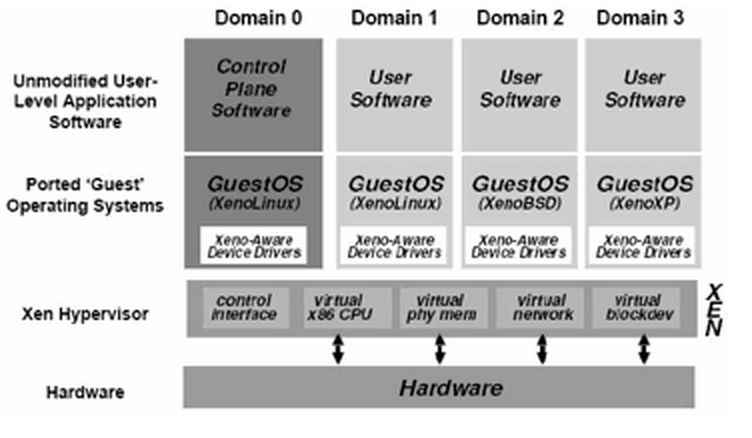
\includegraphics[width=0.5\textwidth]{images/xen}
\end{figure}


\subsection{Redis}

Redis is a type of database often called data structure server and is the most popular key-value store in industry\cite{dbengines}.
Redis maps keys to various types of values, including strings (supported by Keyvee) as well as lists, sets, bitmaps, sorted sets, hash tables and various other data structures.
Its working set and all of its data is in-memory at all times allowing for fast data storage and retrieval.
There is also optional durability either writing the dataset to disk every now and then or using append-only log files.
Redis supports atomic operations on the types it supports, so for example it has commands to append to string and increment stored integers.
Redis is widely used and has various applications in server infrastructure, examples include:

\begin{itemize}
  \item Publish / Subscribe
  \item Queues
  \item Caching
  \item Real time analysis
\end{itemize}

Redis has support for master-slave replication, and allows slaves to be masters to other slaves, enabling Redis to implement single-rooted replication tree.
Redis also has support for clustering as of version 3.0.
When durability is not needed, Redis is very performant, although according to tests it has been shown to spend upward of 84\% of it's processing in kernel space, meaning there is space to improve its performance by decreasing time spent and increasing performance in the OS layer \cite{latency}.
Redis is written in ANSI C and works in most POSIX systems without external dependencies but Linux is recommended for deployment. \cite{redisintroduction}.

\subsection{Unikernels}

In todays real world deployments, Virtual Machines normally contain a full operating-system image like Linux hosting a primary application in user space, for example Redis or PostgreSQL, along with supporting services like syslog or NTP running concurrently.
So although most of these VMs contain flexible layers of software, most of them ultimately perform a single function like acting as a host for database for example.
Since the layers that form these VM contain a lot of unused extraneous software, there is a opportunity for optimization both in terms of performance by adapting a OS to the task it's performing and removing extraneous layers and also by improving security by reducing redundant software, making VM's attack surface smaller.
Modern hypervisors like Xen provide resource multiplexing, becoming more advanced with special virtualization features being developed and supported by new hardware.
By reimplementing some core low level features of traditional operating systems like the TCP/IP stack and a file-system interface and using modern hypervisors to manage resources and provide separation between VM's, we can implement unikernels.

\subsection{Mirage OS}

Mirage OS is an OCaml-based library operating system that originated from the Xen Project.
It allows you to compile applications directly to a Xen hypervisor image thereby creating a unikernel, meaning you can run said applications directly on top of a Xen hypervisor without an intermediary operating system.
This approach yields several performance, implementation and security benefits.
Mirage applications are entirely type-safe due to the strong typing of OCaml and the projects effort to reimplemented frameworks such as TCP/IP and SSL to have end-to-end type safety in the Mirage OS stack.
They also have a very compact size due to the lack of structural libraries that must be included.
With the elimination of an operating system interface layer, Mirage applications achieve top-notch performance as there is no additional layer in the IO pipeline or scheduler to delay the application's execution.

\begin{figure}[ht]
  \centering
  \caption{Mirage OS architecture}
  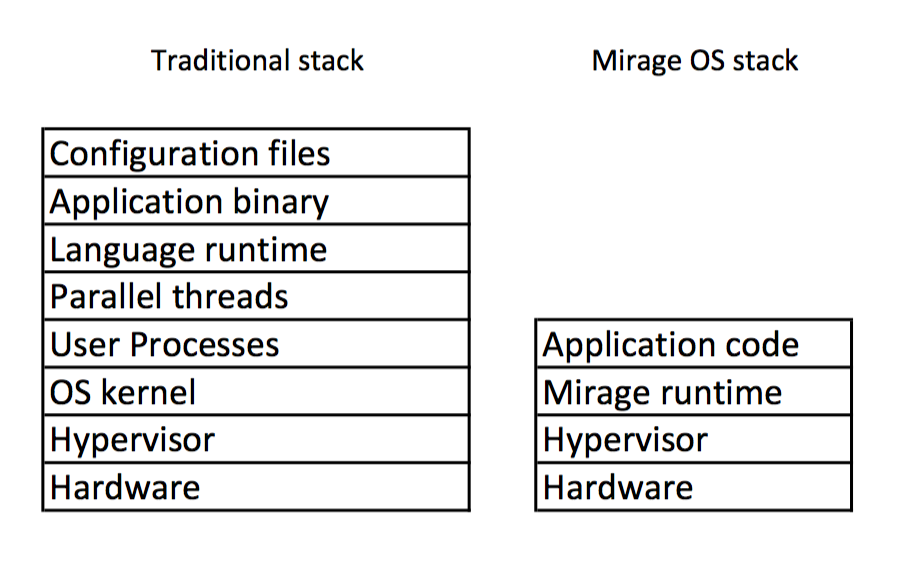
\includegraphics[width=0.5\textwidth]{images/design}
\end{figure}

Thanks to its simple runtime, OCaml, an expressive functional systems programming language, was a good fit for the Mirage project, and was used to re\-implement the runtime in an image that would run on Xen.
The strictness of OCaml's type system ensures that programs are respect with regard to variable data types prior to compilation, because of this strictness the executable is able to shed all type checking which yields fast native code with performance comparable to C.

As highlighted in Figure 1, unikernels have a greatly reduced overhead when accessing resources relative to an application running on Linux.
This approach brings some great benefits like zero-copy IO and no scheduler-induced delay in response.
These performance improvements are important in high throughput and low latency applications like key-value datastores.
However, this approach does have downfalls such as Mirage's limit to a single virtual machine per core; this limitation means that certain applications that require access to multiple physical threads will not fit the Mirage programming model.
For applications that do not need multiple physical threads but need asynchronous IO, Mirage has a lightweight cooperative threading, Lwt, library that provides simple constructs for asynchronous code.

Simple experiments with Mirage have proven that competitive performance to native C applications is not difficult to achieve.
For example, a Mirage DNS server implementation outperformed the standard Bind9 and NSD servers by 14\% in raw throughput in testing.
This indicates that for the right workload, Mirage is an attractive choice that should be evaluated.

In addition to the performance benefits, unikernels are inherently more secure than a standard operating system.
The smaller the attack surface area, the more difficult it is to compromise an application.
In addition, by reimplementing TCP/IP, SSL and more in OCaml, the Mirage OS project aims to make memory safety end-to-end from application code to the lowest level.
When a Mirage image is compiled, only the imported libraries are included which means that only the necessary ports and protocols are exposed.
This aspect, combined with the type-safety OCaml provides eliminates entire classes of security vulnerabilities in Mirage applications.


\section{Design and Implementation}

For Keyvee we have the following goals:

\begin{itemize}
  \item Implement subset of Redis functionality in OCaml on top of the Mirage OS toolchain.
  \item Make Keyvee as compatible to Redis as possible and a drop-in replacement for most purposes.
  \item Implement RESP, Redis's protocol specification, to allow interoperability with existing tools and libraries.
\end{itemize}

Here in this section we will talk about our implementation of Keyvee and how we try to accomplish these goals.

\subsection{Overview}

\begin{center}
\captionof{table}{Supported commands}
  \begin{tabular}{ | l | }
    \hline
    GET <key> \\ \hline
    SET <key> <value> \\ \hline
    DEL <key> \\ \hline
    MGET <key> [<key> ...] \\ \hline
    MSET <key> <value> [<key> <value> ...] \\ \hline
    PING \\ \hline
  \end{tabular}
\end{center}



Keyvee is implemented on top of the Mirage OS toolchain using OCaml.
Currently, we support the GET, SET, DEL, PING, MSET and MGET commands.
All data is stored in-memory, similar to Redis.
We have an internal module implementation built on top of OCaml's Hashtbl module, which stores our keys and associated data in an efficient lookup table.
We use a hash table with a seeded hash function, using a seed randomly chosen at hash table creation time.
This means the hash function is randomly selected among 230 different hash functions with different collision patterns which helps stop denial-of-service attacks where attackers can send input crafted to create collisions, slowing our application to a halt.

Mirage OS has support for the Lwt library which we use extensively, allowing us to support concurrent clients.
Lwt is a cooperative threading library supporting very lightweight threads that cannot be preempted and do not need a new stack or a new process like traditional threads.
While it hinders parallelism in CPU bound applications, it's perfect for an I/O bound application like Keyvee.

At startup, our hashtable is initialized and the server is prepared to receive connections. An Lwt event loop is setup and a listening socket is opened on 6379, Redis's default port.
We use Mirage OS's low level TCP/IP network stack which is implemented in pure OCaml.
When a client attempts to connect, a lightweight Lwt thread is spawned and our command handler commences parsing the RESP string.
When the command has been parsed, either an error is issued if the command is nonsensical or the corresponding internal command is called and return value is encoded back to RESP and sent to the client.
The parse functions fully support well formed queries for our supported functions, but lack some verification steps and will not respond to badly formed queries.
Depending on which internal commands is called, it interfaces with our Hashtbl module to retrieve or write data.

Leveraging Mirage and OCaml guarantees type safety in both our application as well as in the implementations of frameworks underlying the application such as the TCP/IP stack, enhancing the security of our implementation.
Because memory layout in Mirage is used to distinguish I/O pages, the OCaml garbage collector needs to scan less to be as effective as in a full stack OS, which let's the network stack perform predictably.
Predictable performance, as well as support for zero-copy I/O makes Mirage's network stack more performant than traditional full stack OS.

\begin{figure}[ht]
  \centering
  \caption{Example of RESP, Client asking Server for length of "mylist"}
  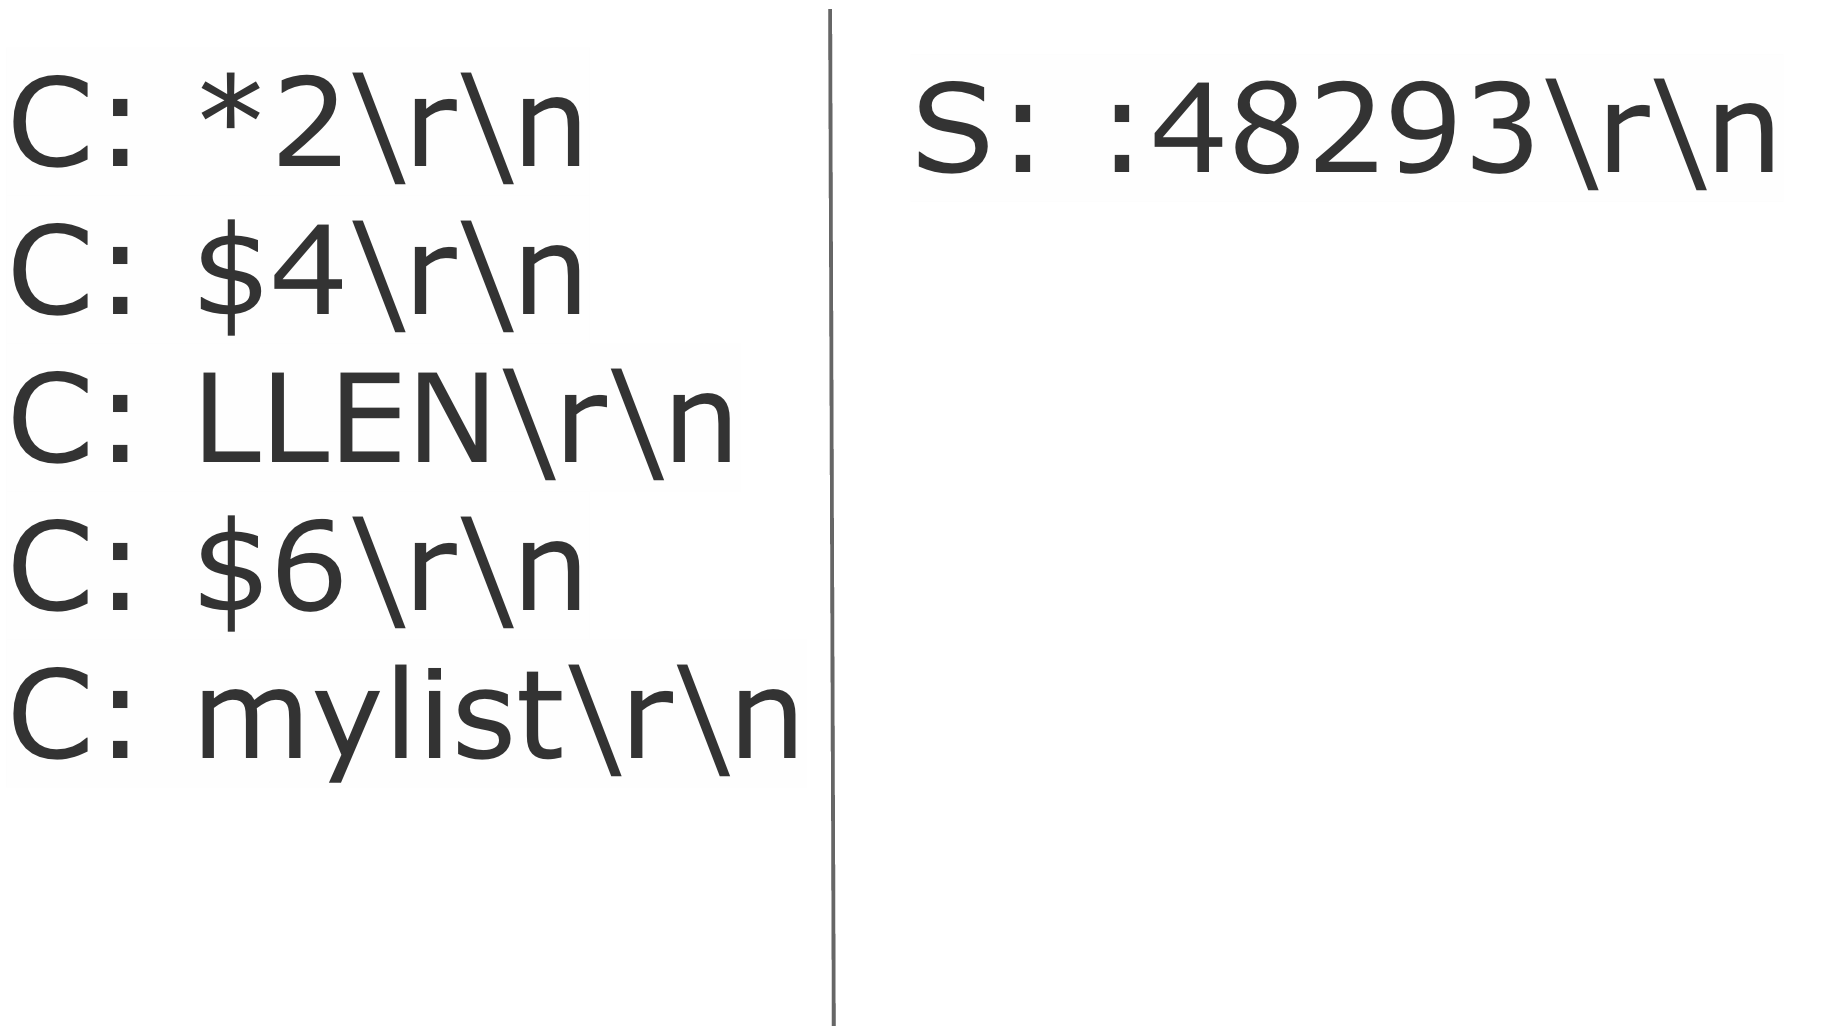
\includegraphics[width=0.5\textwidth]{images/resp}
\end{figure}


\subsection{Redis implementation}

As Redis is a full featured and working database implementation it goes through a lot of steps that Keyvee does not.
It starts by initializing a server state structure, which is where it stores configuration information such as the port it is running on, database files, replication, sort parameters and various other data.
Redis is a well written and organized project and the codebase is straightforward to read despite all the optimizations present.
One such optimization is a pool of shared objects that is created when the server initializes which decreases allocations needed.
The shared objects are for constant replies like PONG and also include allocations for the first 10,000 integers in RESP form. \cite{redisunderthehood}
Redis then creates a event loop, using epoll on Linux and kqueue on BSD and falls back to select if those are not available.
This is what makes Redis so responsive and allows it to be single threaded but still serve thousands of clients simultaneously, and is comparable to what Lwt and the Lwt event engine does for Keyvee.
After setting up the event loop, Redis further initializes databases (it has support for multiple databases), TCP listening socket, sets up a server cron function which is called every 100 milliseconds and handles misc administrative tasks and finally registers a connection handler with the event loop and opens an append-only file if configured to do so.

Redis accepts connections in the event loop using standard POSIX methods, and as RESP is a ASCII based protocol it parses strings to process the commands similarly to how Keyvee does this, albeit it in a very efficient manner.
After parsing the command string, the command is looked up in the internal command table and it's executed.
Write commands such as SET make the server have dirty data so the server is marked as having pages in memory that have changed.
This is then used during the automatic save process and append-only log file writing process.
Redis has some strategies to minimize latency and roundtrips, for example pipelining which is when multiple commands are sent at once to the server, without waiting for acknowledgment or responses for earlier commands.
This is a good strategy and is adopted by Keyvee as well, but we believe that the approach of moving the key-value datastore to a unikernel implementation will yield even greater and more reliable performance.


\subsection{Benefits}

The benefits that can be gained from a Mirage OS implementation of Redis are mainly performance and security benefits.

\subsubsection{Performance}

Although our current test implementation did not exceed Redis's implementation under heavy load, theoretically the Mirage OS implementation should be more performant by making the stack smaller and eliminating the OS networking and scheduling layers. We are certain that with more optimization work Keyvee would become more performant than Redis with equal functionality.

\subsubsection{Security}

There are two security aspects of Mirage OS that are pertinent to our Keyvee implementation.
By only compiling Keyvee into a OS image, a lot of extra services and weak points in traditional OS's are not run, and so with a smaller attack surface certain kinds of vulnerabilities are eliminated.
In addition to minimizing the attack surface, Mirage OS applications are end-to-end memory safe because OCaml's runtime manages memory allocation and reclaims memory with a mature garbage collector.
That means from the TCP/IP stack, up to SSL and the application code, everything is compiled using a memory-safe language which guarantees that Keyvee is completely memory safe.
While Redis is well written and has good test coverage, it cannot be guaranteed to be memory-safe like Keyvee, being written purely in C.
The recommendation for deployment of Redis is to put it behind a firewall, which is both because of lack of user access control (anyone can for example issue FLUSHDB and remove all data from server) but another concern is the lack of memory safety.
This means Redis is vulnerable to buffer overflow and out of bounds errors for example which have been the main sources of vulnerabilities in server software, latest notable example being the Heartbleed bug.
Meanwhile, Keyvee is completely memory safe and with addition of user access controls could be trusted enough to be fully exposed on the internet, which opens it up to a whole host of applications that Redis could only handle by having a server as a intermediary.
For example, a mobile client could connect directly to Keyvee for data that needs no server processing instead of going through a intermediary server.

\subsubsection{Immutable infrastructure}

Immutable infrastructure consists of immutable components that are replaced in every deployment rather than being simply updated in place.
Those components are started from an image that is built once per deployment and can then be tested and validated before being deployed.
Traditionally, full stack operating systems are deployed to run applications and then updated regularly, but this can be unreliable as updates can break the running application.
As Keyvee is a unikernel which are immutable applications, Keyvee can be a component in an immutable infrastructure.

\subsection{Development process}

We use distributed version control system Git and Github to track changes to our codebase.
Travis Continuous Integration is then used to build our codebase when changes are made and check for any errors.
It is possible to build a Unix binary using the Mirage toolchain, which we use extensively when developing our code before it is deployed and tested on the Xen server.

The Mirage OS documentation leaves a lot to be desired and many times we needed to go looking into Mirage OS's implementation it self.
In addition, some OCaml modules do not work with the toolchain and there is scarcity of open source code built with it.
Especially as it is the early days there is not a lot of community support surrounding Mirage.


\section{Evaluation}
\subsection{Testing Environment}
We performed all of our evaluations on a dedicated 8-core HP ProLiant rack server with 16 GB RAM available.
Our Xen hypervisor installation is coordinated by a Ubuntu Server 14.04 host that serves as the management domain to manage the other hosts running on the Hypervisor.
The Mirage installation was modified to use Redis's communication protocols so that we could use the same benchmark for all test setups. The benchmark was run using 50 parallel clients sending a 3-byte payload.
The Redis setups were given ten thousands requests as part of their benchmark, while the Mirage setups on Xen were given five hundred, one thousand, or ten thousand requests.

\subsection{Running Mirage}


When a MirageOS unikernel is configured in Xen mode, both the unikernel image and the configuration file are generated.
With these, a unikernel can be easily launched using the xl Xen management tool.
Due to the small size of the image, this is a quick process where the Mirage image configures itself when started by xl.
We used a Redis 2.8 installation on Xen as the comparison application to Keyvee.
The test clients were hosted by the supervising host on Xen.

Using the Redis benchmark suite to examine Keyvee provided guarantees that the Redis communication protocols were properly fulfilled and provided a common means of measuring throughput.
The distribution of command latency was also recorded, as it was automatically provided by the benchmark suite.
Four commands were implemented and tested: SET, which assigned a single key its value; MSET, which assigned values to multiple keys; GET, which retrieves the value of a given key; and PING, which tests the server's connectivity.

Three aspects of scalability were tested: raw request volume, request parallelization, and request pipelining.
To test scalability with raw volume, a benchmark setup would have either a total of one million or five million of each command.
For parallelization, the remote host would set up a group of 10, 100, 500, one thousand clients.
Regarding pipelining, requests were pipelined by sending 1, 10, or 50 commands sent per request.
Individual keys were 20 bytes large, and the number of keys used in a given test was equal to the number of total requests divided by one hundred.
Each benchmark setup used a combination of these three aspects, resulting in a total of 16 unique tests.

\subsection{Overall Performance}

Increasing the number of total requests had no significant effect on the relative throughput of Keyvee when compared to Redis.
Throughput increases through pipelining proved to scale better with Keyvee, but its benefit was usually overtaken by the profound effect scaling the number of concurrent clients had on throughput.
Except for one of the implemented commands, Keyvee performed just as well, if not better, than Redis when only ten were connecting at once.
However, Keyvee's throughput decreased logarithmically as the number of simultaneous clients increased, while Redis would only have a slight linear decrease, if at all.
This meant that Keyvee would usually have consistently lower throughput than Redis after a certain low threshold, with some variance between commands.
Upon further examination of the code and testing, it was found that the overhead from the light-weight threads used by Mirage to handle simultaneous connections resulted in the severely reduced throughput.
With regards to the latency, each test showed a similar pattern, with Keyvee tending to have a much wider distribution, caused mainly by having a low number of commands taking an extraordinary amount of time.

\subsection{SET Command}

\begin{figure}[!htb]
\begin{tikzpicture}[scale=0.9]
\begin{axis}[
xlabel = {Parallel Clients},
ylabel = {Throughput (10\textsuperscript{5} Requests/sec)},
legend columns = 3,
transpose legend,
legend style={at={(0.5,-0.2)},anchor=north}]
\addplot[
color=cyan,
mark=diamond,
]
table{./results/redis/SET__pipeline_1_.results};
\addlegendentry{Redis, no pipeline};
\addplot[
color=cyan,
mark=square,
]
table{./results/redis/SET__pipeline_10_.results};
\addlegendentry{Redis, pipeline of 10};
\addplot[
color=cyan,
mark=triangle,
]
table{./results/redis/SET__pipeline_50_.results};
\addlegendentry{Redis, pipeline of 50};
\addplot[
color=red,
mark=diamond,
]
table{./results/keyvee/SET__pipeline_1_.results};
\addlegendentry{Keyvee, no pipeline};
\addplot[
color=red,
mark=square,
]
table{./results/keyvee/SET__pipeline_10_.results};
\addlegendentry{Keyvee, pipeline of 10};
\addplot[
color=red,
mark=triangle,
]
table{./results/keyvee/SET__pipeline_50_.results};
\addlegendentry{Keyvee, pipeline of 50};
\end{axis}
\end{tikzpicture}
\caption{SET Throughput\label{fig:SET_T}}
\end{figure}

\begin{figure}[!htb]
\begin{tikzpicture}[scale=0.9]
\begin{axis}[
xmode = log,
xlabel = {Maximum completion time},
ylabel = {Percent of all requests},
legend columns = 4,
transpose legend,
legend style={at={(0.5,-0.2)}, anchor=north}]
	\addplot[
	color=cyan,
	mark=diamond,
	]
	table{./results/redis/SET_pipeline_1_w_10.cdf.results};
	\addlegendentry{Redis, 10 clients};
	\addplot[
	color=cyan,
	mark=square,
	]
	table{./results/redis/SET_pipeline_1_w_100.cdf.results};
	\addlegendentry{Redis, 100 clients};
	\addplot[
	color=cyan,
	mark=triangle,
	]
	table{./results/redis/SET_pipeline_1_w_500.cdf.results};
	\addlegendentry{Redis, 500 clients};
	\addplot[
	color=cyan,
	mark=star,
	]
	table{./results/redis/SET_pipeline_1_w_1000.cdf.results};
	\addlegendentry{Redis, 1000 clients};
	\addplot[
	color=red,
	mark=diamond,
	]
	table{./results/keyvee/SET_pipeline_1_w_10.cdf.results};
	\addlegendentry{Keyvee, 10 clients};
	\addplot[
	color=red,
	mark=square,
	]
	table{./results/keyvee/SET_pipeline_1_w_100.cdf.results};
	\addlegendentry{Keyvee, 100 clients};
	\addplot[
	color=red,
	mark=triangle,
	]
	table{./results/keyvee/SET_pipeline_1_w_500.cdf.results};
	\addlegendentry{Keyvee, 500 clients};
	\addplot[
	color=red,
	mark=star,
	]
	table{./results/keyvee/SET_pipeline_1_w_1000.cdf.results};
	\addlegendentry{Keyvee, 1000 clients};
	\end{axis}
	\end{tikzpicture}
	\caption{SET Latency w/o pipelining\label{fig:SET_L}}
\end{figure}

As seen in \ref{fig:SET_T}, without pipelining, SET throughput was roughly equal when there were few concurrent clients, but as pipelining increased, Keyvee's throughput improved significantly.
However, gains from pipelining would be eventually offset by the scaling issues of handling concurrent clients.
Interestingly, at a pipeline length of 10 the biggest difference in scaling was found, since the benefits for a 50-long pipeline managed to maintain Keyvee's throughput somewhat.
When comparing latency of the commands, Keyvee's latency only slightly behind Redis, but as the number of concurrent clients grew, the disparity in latency grew wider.

\subsection{MSET Command}

\begin{figure}[!htb]
\begin{tikzpicture}[scale=0.9]
\begin{axis}[
xlabel = {Parallel Clients},
ylabel = {Throughput (10\textsuperscript{4} Requests/sec)},
legend columns = 3,
transpose legend,
legend style={at={(0.5,-0.2)},anchor=north}]
\addplot[
color=cyan,
mark=diamond,
]
table{./results/redis/MSET__10_keys___pipeline_1_.results};
\addlegendentry{Redis, no pipeline};
\addplot[
color=cyan,
mark=square,
]
table{./results/redis/MSET__10_keys___pipeline_10_.results};
\addlegendentry{Redis, pipeline of 10};
\addplot[
color=cyan,
mark=triangle,
]
table{./results/redis/MSET__10_keys___pipeline_50_.results};
\addlegendentry{Redis, pipeline of 50};
\addplot[
color=red,
mark=diamond,
]
table{./results/keyvee/MSET__10_keys___pipeline_1_.results};
\addlegendentry{Keyvee, no pipeline};
\addplot[
color=red,
mark=square,
]
table{./results/keyvee/MSET__10_keys___pipeline_10_.results};
\addlegendentry{Keyvee, pipeline of 10};
\addplot[
color=red,
mark=triangle,
]
table{./results/keyvee/MSET__10_keys___pipeline_50_.results};
\addlegendentry{Keyvee, pipeline of 50};
\end{axis}
\end{tikzpicture}
\caption{MSET Throughput\label{fig:MSET_T}}
\end{figure}
\begin{figure}[!htb]
\begin{tikzpicture}[scale=0.9]
\begin{axis}[
xmode = log,
xlabel = {Maximum completion time},
ylabel = {Percent of all requests},
legend columns = 4,
transpose legend,
legend style={at={(0.5,-0.2)}, anchor=north}]
	\addplot[
	color=cyan,
	mark=diamond,
	]
	table{./results/redis/MSET_10_keys__pipeline_1_w_10.cdf.results};
	\addlegendentry{Redis, 10 clients};
	\addplot[
	color=cyan,
	mark=square,
	]
	table{./results/redis/MSET_10_keys__pipeline_1_w_100.cdf.results};
	\addlegendentry{Redis, 100 clients};
	\addplot[
	color=cyan,
	mark=triangle,
	]
	table{./results/redis/MSET_10_keys__pipeline_1_w_500.cdf.results};
	\addlegendentry{Redis, 500 clients};
	\addplot[
	color=cyan,
	mark=star,
	]
	table{./results/redis/MSET_10_keys__pipeline_1_w_1000.cdf.results};
	\addlegendentry{Redis, 1000 clients};
	\addplot[
	color=red,
	mark=diamond,
	]
	table{./results/keyvee/MSET_10_keys__pipeline_1_w_10.cdf.results};
	\addlegendentry{Keyvee, 10 clients};
	\addplot[
	color=red,
	mark=square,
	]
	table{./results/keyvee/MSET_10_keys__pipeline_1_w_100.cdf.results};
	\addlegendentry{Keyvee, 100 clients};
	\addplot[
	color=red,
	mark=triangle,
	]
	table{./results/keyvee/MSET_10_keys__pipeline_1_w_500.cdf.results};
	\addlegendentry{Keyvee, 500 clients};
	\addplot[
	color=red,
	mark=star,
	]
	table{./results/keyvee/MSET_10_keys__pipeline_1_w_1000.cdf.results};
	\addlegendentry{Keyvee, 1000 clients};
	\end{axis}
	\end{tikzpicture}
	\caption{MSET Latency w/o pipelining\label{fig:MSET_L}}
\end{figure}

Compared to SET, MSET is slightly more complex and time consuming command, resulting in lower throughput for both applications, as seen in Figure \ref{fig:MSET_T}.
It was here that Keyvee always had a lower throughput than Redis, even at low number of concurrent clients.
The disparity in performance became increasingly dramatic as the pipeline length increased and was one of the few areas where pipelining's scaling with Keyvee had little effect.
Most notable how severe diminishing returns pipelining had on both applications; the difference between a pipeline of 10 and 50 was very small, even more so when looking at Keyvee.
As with the SET command, Keyvee's latency became increasingly greater as the number of connected clients increased.

\subsection{GET Command}

\begin{figure}[!htb]
\begin{tikzpicture}[scale=0.9]
\begin{axis}[
xlabel = {Parallel Clients},
ylabel = {Throughput (10\textsuperscript{5} Requests/sec)},
legend columns = 3,
transpose legend,
legend style={at={(0.5,-0.2)},anchor=north}]
\addplot[
color=cyan,
mark=diamond,
]
table{./results/redis/GET__pipeline_1_.results};
\addlegendentry{Redis, no pipeline};
\addplot[
color=cyan,
mark=square,
]
table{./results/redis/GET__pipeline_10_.results};
\addlegendentry{Redis, pipeline of 10};
\addplot[
color=cyan,
mark=triangle,
]
table{./results/redis/GET__pipeline_50_.results};
\addlegendentry{Redis, pipeline of 50};
\addplot[
color=red,
mark=diamond,
]
table{./results/keyvee/GET__pipeline_1_.results};
\addlegendentry{Keyvee, no pipeline};
\addplot[
color=red,
mark=square,
]
table{./results/keyvee/GET__pipeline_10_.results};
\addlegendentry{Keyvee, pipeline of 10};
\addplot[
color=red,
mark=triangle,
]
table{./results/keyvee/GET__pipeline_50_.results};
\addlegendentry{Keyvee, pipeline of 50};
\end{axis}
\end{tikzpicture}
\caption{GET Throughput\label{fig:GET_T}}
\end{figure}
\begin{figure}[!htb]
\begin{tikzpicture}[scale=0.9]
\begin{axis}[
xmode = log,
xlabel = {Maximum completion time},
ylabel = {Percent of all requests},
legend columns = 4,
transpose legend,
legend style={at={(0.5,-0.2)}, anchor=north}]
	\addplot[
	color=cyan,
	mark=diamond,
	]
	table{./results/redis/GET_pipeline_1_w_10.cdf.results};
	\addlegendentry{Redis, 10 clients};
	\addplot[
	color=cyan,
	mark=square,
	]
	table{./results/redis/GET_pipeline_1_w_100.cdf.results};
	\addlegendentry{Redis, 100 clients};
	\addplot[
	color=cyan,
	mark=triangle,
	]
	table{./results/redis/GET_pipeline_1_w_500.cdf.results};
	\addlegendentry{Redis, 500 clients};
	\addplot[
	color=cyan,
	mark=star,
	]
	table{./results/redis/GET_pipeline_1_w_1000.cdf.results};
	\addlegendentry{Redis, 1000 clients};
	\addplot[
	color=red,
	mark=diamond,
	]
	table{./results/keyvee/GET_pipeline_1_w_10.cdf.results};
	\addlegendentry{Keyvee, 10 clients};
	\addplot[
	color=red,
	mark=square,
	]
	table{./results/keyvee/GET_pipeline_1_w_100.cdf.results};
	\addlegendentry{Keyvee, 100 clients};
	\addplot[
	color=red,
	mark=triangle,
	]
	table{./results/keyvee/GET_pipeline_1_w_500.cdf.results};
	\addlegendentry{Keyvee, 500 clients};
	\addplot[
	color=red,
	mark=star,
	]
	table{./results/keyvee/GET_pipeline_1_w_1000.cdf.results};
	\addlegendentry{Keyvee, 1000 clients};
	\end{axis}
	\end{tikzpicture}
	\caption{GET Latency w/o pipelining\label{fig:GET_L}}
\end{figure}
The GET command is simpler than SET, and so Keyvee's throughput, shown in Figure \ref{fig:GET_T}, was relatively better when compared to the SET command.
While it showed similar relative performance to SET when the pipeline was short, there was a higher threshold for when benefit from pipelining was negated by the problems with handling multiple clients; even at 500 clients performance was nearly equal.

\subsection{PING Command}

\begin{figure}[!htb]
\begin{tikzpicture}[scale=0.9]
\begin{axis}[
xlabel = {Parallel Clients},
ylabel = {Throughput (10\textsuperscript{5} Requests/sec)},
legend columns = 3,
transpose legend,
legend style={at={(0.5,-0.2)},anchor=north}]
\addplot[
color=cyan,
mark=diamond,
]
table{./results/redis/PING_BULK__pipeline_1_.results};
\addlegendentry{Redis, no pipeline};
\addplot[
color=cyan,
mark=square,
]
table{./results/redis/PING_BULK__pipeline_10_.results};
\addlegendentry{Redis, pipeline of 10};
\addplot[
color=cyan,
mark=triangle,
]
table{./results/redis/PING_BULK__pipeline_50_.results};
\addlegendentry{Redis, pipeline of 50};
\addplot[
color=red,
mark=diamond,
]
table{./results/keyvee/PING_BULK__pipeline_1_.results};
\addlegendentry{Keyvee, no pipeline};
\addplot[
color=red,
mark=square,
]
table{./results/keyvee/PING_BULK__pipeline_10_.results};
\addlegendentry{Keyvee, pipeline of 10};
\addplot[
color=red,
mark=triangle,
]
table{./results/keyvee/PING_BULK__pipeline_50_.results};
\addlegendentry{Keyvee, pipeline of 50};
\end{axis}
\end{tikzpicture}
\caption{PING Throughput\label{fig:PING_T}}
\end{figure}
\begin{figure}[!htb]
\begin{tikzpicture}[scale=0.9]
\begin{axis}[
xmode = log,
xlabel = {Maximum completion time},
ylabel = {Percent of all requests},
legend columns = 4,
transpose legend,
legend style={at={(0.5,-0.2)}, anchor=north}]
	\addplot[
	color=cyan,
	mark=diamond,
	]
	table{./results/redis/PING_BULK_pipeline_50_w_10.cdf.results};
	\addlegendentry{Redis, 10 clients};
	\addplot[
	color=cyan,
	mark=square,
	]
	table{./results/redis/PING_BULK_pipeline_50_w_100.cdf.results};
	\addlegendentry{Redis, 100 clients};
	\addplot[
	color=cyan,
	mark=triangle,
	]
	table{./results/redis/PING_BULK_pipeline_50_w_500.cdf.results};
	\addlegendentry{Redis, 500 clients};
	\addplot[
	color=cyan,
	mark=star,
	]
	table{./results/redis/PING_BULK_pipeline_50_w_1000.cdf.results};
	\addlegendentry{Redis, 1000 clients};
	\addplot[
	color=red,
	mark=diamond,
	]
	table{./results/keyvee/PING_BULK_pipeline_50_w_10.cdf.results};
	\addlegendentry{Keyvee, 10 clients};
	\addplot[
	color=red,
	mark=square,
	]
	table{./results/keyvee/PING_BULK_pipeline_50_w_100.cdf.results};
	\addlegendentry{Keyvee, 100 clients};
	\addplot[
	color=red,
	mark=triangle,
	]
	table{./results/keyvee/PING_BULK_pipeline_50_w_500.cdf.results};
	\addlegendentry{Keyvee, 500 clients};
	\addplot[
	color=red,
	mark=star,
	]
	table{./results/keyvee/PING_BULK_pipeline_50_w_1000.cdf.results};
	\addlegendentry{Keyvee, 1000 clients};
	\end{axis}
	\end{tikzpicture}
	\caption{PING Latency with a pipeline of 50\label{fig:PING_L}}
\end{figure}
The PING command was the simplest command to implement because PING commands never referenced the internal datastore and have a static response of "PONG".
Because of this simplicity, it heavily benefited from the scaling that pipelining provided.
This resulted in results that broke the usual performance patterns, shown in Figure \ref{fig:PING_T}.
Most notably, while it still showed the logarithmic performance loss like all the other commands, the tests done with a pipeline size of 50 showed Keyvee consistently having a much higher throughput than Redis.
However, at shorter pipeline stages, the performance of PING for both applications were none too different than their performance with SET.
Similarly, the latency at short pipeline sizes was unremarkable.
However, as shown in Figure \ref{fig:PING_L}, at the larger pipeline sizes, Keyve was found to have a more gradual distribution curve, verses Redis' steep cliffs.
Furthermore, Keyvee had less commands that took an extreme amount of time when compared to the other command types.

\section{Conclusion}
In this paper we described the implementation and evaluation of our unikernel key-value store, Keyvee.
Our efforts are concentrated around implementing a subset of Redis's functionality using OCaml and the Mirage OS toolchain.
We then evaluated our implementation and compared it with Redis using Redis's benchmarking tool.
While similar, if not superior, throughput was generally achieved in tests having few parallel clients, a scaling issue was found when Keyvee was subjected to larger parallel loads, resulting in poor throughput.
The main source of the low throughput was identified as an underlying issue with Mirage OS's difficulty in handling large numbers of multiple clients, however, we believe that this problem will be addressed as Xen, and unikernels as a whole, mature as a technology.

\section{Lessons learned}
The project was a great lesson and deepened our knowledge in low level operating systems constructs and virtualization.
Due to features like high reliability and great tooling, OCaml can be a good tool to create systems software similar to Mirage OS.
Lwt did not prove as mature as kqueue and epoll in our testing.
There are some bugs present in the Unix implementation of Mirage, meaning one can not fully rely on compiling a Unix version of Mirage OS but highlights the need to build a Xen image for testing to get a true image of how the application would behave in production.

\section{Future work}
Our project implements the basics of Redis which allowed us to evaluate the viability of our idea.
Future work would include finishing implementing the rest of Redis's data structures and data operations, data persistance as well as some of the advanced features like clustering and replication.
In addition to achieving Redis's featureset, there is potential in Keyvee to have additional features thanks to the unique development toolchain.
An example is implementing user access control and other precautions that would allow Keyvee to expose a listening socket to the internet, allowing clients to connect directly to our database without intermediary server.

\section{Acknowledgements}


We thank the kind souls in the \#Mirage and \#Xen IRC chatroom for their relentless patience.
Their assistance was crucial in learning how to use Mirage's utilities and leverage the provided standard library as well as learning how to actually launch our completed product on Xen.



\bibliographystyle{abbrv}
\bibliography{bibliography}


\end{document}



